\documentclass{physlab}

\begin{document}
\begin{titlepage}
\center % Center everything on the page
 
%----------------------------------------------------------------------------------------
%	HEADING SECTIONS
%----------------------------------------------------------------------------------------

\textsc{\LARGE Московский\\[-0.2cm]Физико-Технический Институт\\[0.1cm]\large (государственный университет)}\\[1.5cm] % Name of your university/college
\textsc{\Large Кафедра общей физики}\\[0.1cm] % Major heading such as course name
\textsc{\large Лабораторная работа № 3.1.1}\\[0.5cm] % Minor heading such as course title

%----------------------------------------------------------------------------------------
%	TITLE SECTION
%----------------------------------------------------------------------------------------

\HRule
\\[0.6cm]
{ \huge \bfseries Магнитометр}
\\[0.3cm] % Title of your document
\HRule
\\[1.5cm]


 
%----------------------------------------------------------------------------------------
%	AUTHOR SECTION
%----------------------------------------------------------------------------------------

\begin{minipage}[t]{0.48\textwidth}
	\begin{flushleft} \large
		\textsf{Студент}\bigskip
		
		\tline{(имя)}{30mm} \tline{(фамилия)}{45mm} \\[5mm]
		\underline{\hspace{30mm}} группа
	\end{flushleft}
\end{minipage}
\hfill
\begin{minipage}[t]{0.48\textwidth}
	\begin{flushright} \large
		\textsf{Преподаватель}\bigskip
		
		\tline{(имя)}{30mm} \tline{(отчество)}{45mm} \\[5mm]
		\tline{(фамилия)}{45mm}
	\end{flushright}
\end{minipage}

\begin{bottompar}
	\begin{center}
		
\includegraphics[width = 80 mm]{logo.jpg}
	\end{center}
	\tline{(дата)}{80mm}

\end{bottompar}
\vfill % Fill the rest of the page with whitespace

\end{titlepage}
\textbf{Цель работы:} Изучить влияние активного сопротивления, индуктивности и емкости на сдвиг фаз между током и напряжением в цепи переменного тока.

\section{Экспериментальная установка}



\begin {figure}[H]
\begin{center}
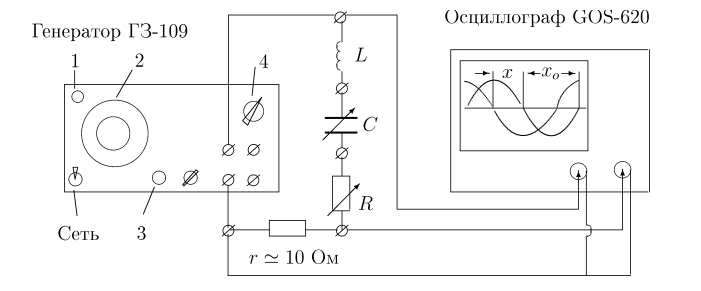
\includegraphics[width=0.9\tw]{t}
\end{center}
\end {figure}
$$R_L= \val \text{при $\nu = $}$$
$$L = $$
$$r = $$
$$C = $$
$$\nu = $$

\subsection*{RC-цепь}

Ток, текущий через RC цепочку, пропорционален напряжению на резисторе, и опережает напряжение на конденсаторе по фазе на $\pi/2$. В таком простом случае метод векторных диаграмм даёт простой результат для зависимости сдвига фаз от $R$:
$$\tg \varphi = \frac{1}{\Omega R C}$$
\begin {figure}[H]
\begin{center}
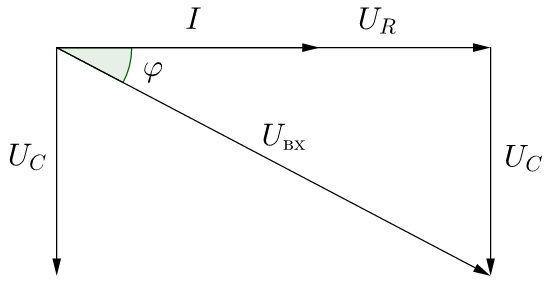
\includegraphics[width=0.6\tw]{rcd}
\end{center}
\end {figure}

\subsection*{RL-цепь}

Всё аналогично RC цепочке, только импеданс катушки теперь 
$$Z_2 = j\omega L,$$
поэтому ток отстаёт по фазе от напряжения, а рассчётная формула приобретает вид
$$\tg \varphi = \frac{\omega L}{R_{\sum}}$$
Теперь к сопротивлению калибровочного резистора и резистора $R$ добавится активное сопротивление катушки:
$$R_{\sum} = R+r+R_L,$$
где $R_L$ -- активное сопротивление катушки.

\subsection*{RCL-цепь}

Комплексный импеданс RCL-цепочки:
$$Z=R+j\omega L - \frac{j}{\omega C}.$$

Сдвиг фаз между током и напряжением получим, взяв аргумент $Z$:

$$\tg\varphi = \frac{\omega L - \frac{1}{\omega C}}{R} = Q\frac{\left(\frac{\omega}{\omega_0}\right)^2 - 1}{\frac{\omega}{\omega_0}} = Q\frac{(1+x)^2-1}{1+x} \simeq 2x Q,$$
где $x = \Delta \omega / \omega_0 = \Delta \nu / \nu_0$, и в последнем переходе пренебрегаем квадратичными по $x$ членами.
Измерив ширину графика $w=2x$ на высоте $\varphi = \pi / 4\ (\tg\varphi = 1)$, можем непосредственно измерить добротность контура:
$$Q = \frac{1}{w}$$

\subsection*{Фазовращатель}

\begin {figure}[H]
\begin{center}
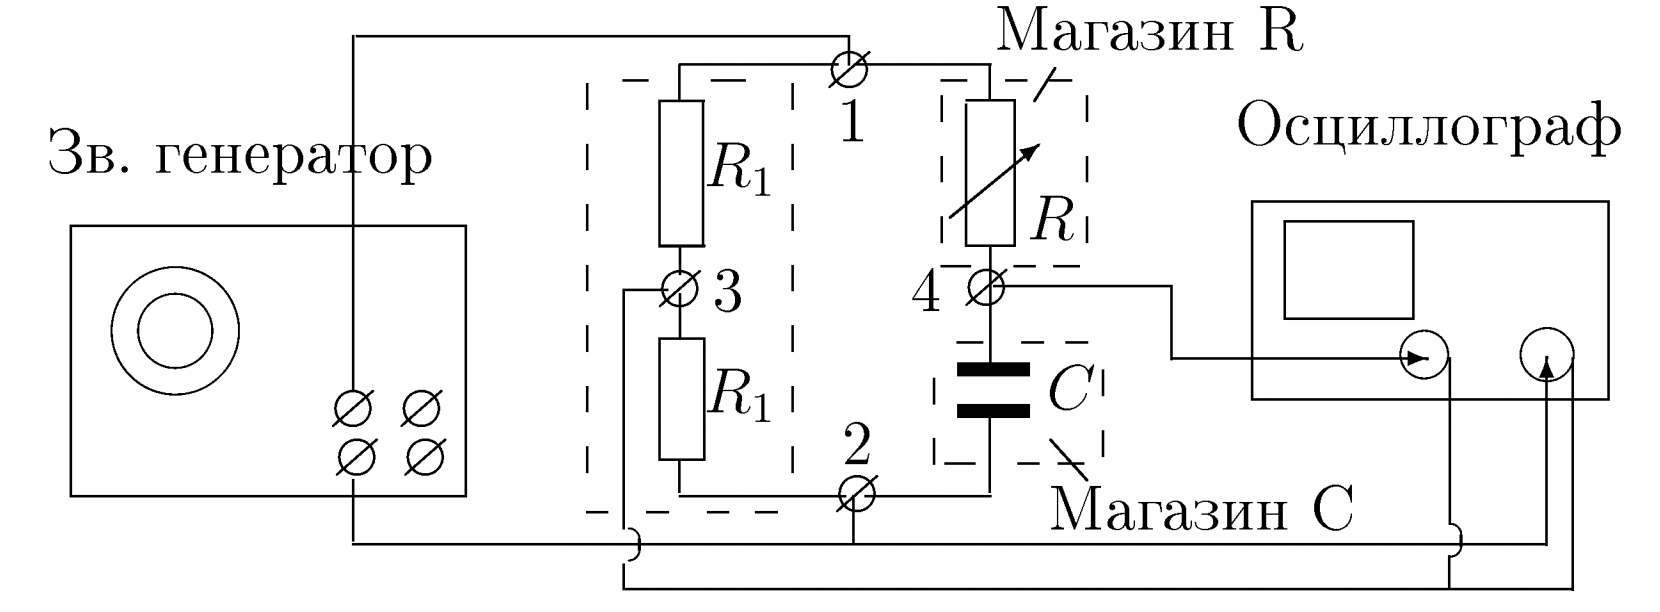
\includegraphics[width=0.8\tw]{phase.png}
\end{center}
\end {figure}


\begin {figure}[H]
\begin{center}
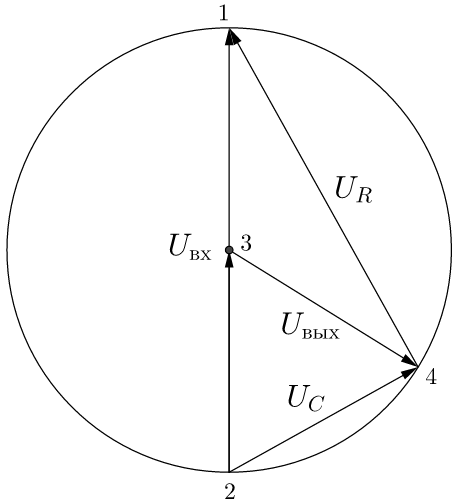
\includegraphics[width=0.7\tw]{diagramphase}
\end{center}
\end {figure}

Разность фаз равна $\pi /2$, когда медиана $34$ является и высотой, т.е. когда $\triangle 124$ -- равнобедренный, откуда

\section{Работа и измерения}

\subsection*{RC-цепь}

$$X_1 = \dfrac{1}{2 \pi \nu C} = $$

\begin{table}[H]
\centering
\begin{tabular}{|c|c|c|c|c|c|c|}
\hline
$R$ & $x$ & $x_0$ & $\varphi$ & $\tg \varphi$ & $R_{\Sigma}$ & $1/(R_{\Sigma} \Omega C)$ \\ \hline
\val    &    \val   &   \val    &   \val    &   \val    &   \val    &   \val    \\ \hline
\val    &    \val   &   \val    &   \val    &   \val    &   \val    &   \val    \\ \hline
\val    &    \val   &   \val    &   \val    &   \val    &   \val    &   \val    \\ \hline
\val    &    \val   &   \val    &   \val    &   \val    &   \val    &   \val    \\ \hline
\val    &    \val   &   \val    &   \val    &   \val    &   \val    &   \val    \\ \hline
\val    &    \val   &   \val    &   \val    &   \val    &   \val    &   \val    \\ \hline
\val    &    \val   &   \val    &   \val    &   \val    &   \val    &   \val    \\ \hline
\val    &    \val   &   \val    &   \val    &   \val    &   \val    &   \val    \\ \hline
\val    &    \val   &   \val    &   \val    &   \val    &   \val    &   \val    \\ \hline
\val    &    \val   &   \val    &   \val    &   \val    &   \val    &   \val    \\ \hline
\val    &    \val   &   \val    &   \val    &   \val    &   \val    &   \val    \\ \hline
\val    &    \val   &   \val    &   \val    &   \val    &   \val    &   \val    \\ \hline
\val    &    \val   &   \val    &   \val    &   \val    &   \val    &   \val    \\ \hline
\val    &    \val   &   \val    &   \val    &   \val    &   \val    &   \val    \\ \hline
\end{tabular}
\caption{Полученные значения в RC-цепи}
\end{table}

Найдем погрешности измерения величин:
$$\sigma_{\tg \varphi} = 
0.1\pi \sqrt{\left(\dfrac{1}{x_0 \cos^2\left(\dfrac{\pi x}{x_0}\right)}\right)^2 + \left(\dfrac{x}{x_0^2 \cos^2 \left(\dfrac{\pi x}{x_0}\right)}\right)^2} $$

	\begin {figure}[H]
		\begin{center}
			
\includegraphics[width=0.7\tw]{foo}
			\caption{График зависимости $\tg \varphi = f[1/ \Omega C R_{\Sigma}]$}
		\end{center}
	\end {figure}

\subsection*{RL-цепь}
\[X_2 = 2 \pi \nu L = \]

\begin{table}[H]
\centering
\begin{tabular}{|c|c|c|c|c|c|c|}
\hline
$R $ & $x$  & $x_0$ & $\varphi$ & $\tg \varphi$ & $R_{\Sigma}$ & $\Omega L/ R_{\Sigma} $ \\ \hline
\val & \val & \val  & \val      & \val          & \val         & \val                  \\ \hline
\val & \val & \val  & \val      & \val          & \val         & \val                  \\ \hline
\val & \val & \val  & \val      & \val          & \val         & \val                  \\ \hline
\val & \val & \val  & \val      & \val          & \val         & \val                  \\ \hline
\val & \val & \val  & \val      & \val          & \val         & \val                  \\ \hline
\val & \val & \val  & \val      & \val          & \val         & \val                  \\ \hline
\val & \val & \val  & \val      & \val          & \val         & \val                  \\ \hline
\val & \val & \val  & \val      & \val          & \val         & \val                  \\ \hline
\val & \val & \val  & \val      & \val          & \val         & \val                  \\ \hline
\end{tabular}
\caption{Полученные значения в RL-цепи}
\end{table}

\begin {figure}[H]
	\begin{center}
		
\includegraphics[width=0.8\tw]{foo}
		\caption{График зависимости $\tg \varphi = f[\Omega L / R_{\Sigma}]$}
	\end{center}
\end {figure}

\subsection*{RCL-цепь}

\begin{table}[H]
\centering
\begin{tabular}{|c|c|c|c|c|c|}
\hline
Сопротивление & $\nu, \text{кГц}$ & $x_0$ & $x$ & $\varphi$ & $nu\nu_0$ \\ \hline
\multirow{11}{*}{$R = 0 \text{ Ом}$}     & \val            & \val   & \val & \val   & \val      \\ \cline{2-6} 
                                         & \val            & \val   & \val & \val   & \val      \\ \cline{2-6}
                                         & \val            & \val   & \val & \val   & \val      \\ \cline{2-6}
                                         & \val            & \val   & \val & \val   & \val      \\ \cline{2-6}
                                         & \val            & \val   & \val & \val   & \val      \\ \cline{2-6}
                                         & \val            & \val   & \val & \val   & \val      \\ \cline{2-6}
                                         & \val            & \val   & \val & \val   & \val      \\ \cline{2-6}
                                         & \val            & \val   & \val & \val   & \val      \\ \cline{2-6}
                                         & \val            & \val   & \val & \val   & \val      \\ \cline{2-6}
                                         & \val            & \val   & \val & \val   & \val      \\ \cline{2-6}
                                         & \val            & \val   & \val & \val   & \val      \\ \cline{2-6}
                                         & \val            & \val   & \val & \val   & \val      \\ \hline
\multirow{13}{*}{$R = 100 \text{ Ом}$}   & \val            & \val   & \val & \val   & \val      \\ \cline{2-6} 
                                         & \val            & \val   & \val & \val   & \val      \\ \cline{2-6}
                                         & \val            & \val   & \val & \val   & \val      \\ \cline{2-6}
                                         & \val            & \val   & \val & \val   & \val      \\ \cline{2-6}
                                         & \val            & \val   & \val & \val   & \val      \\ \cline{2-6}
                                         & \val            & \val   & \val & \val   & \val      \\ \cline{2-6}
                                         & \val            & \val   & \val & \val   & \val      \\ \cline{2-6}
                                         & \val            & \val   & \val & \val   & \val      \\ \cline{2-6}
                                         & \val            & \val   & \val & \val   & \val      \\ \cline{2-6}
                                         & \val            & \val   & \val & \val   & \val      \\ \cline{2-6}
                                         & \val            & \val   & \val & \val   & \val      \\ \cline{2-6}
                                         & \val            & \val   & \val & \val   & \val      \\ \hline
\end{tabular}
\caption{Полученные значения при изучении зависимости фазы от $\dfrac{\nu}{\nu_0}$}
\end{table}

\[C = \val, \; L = \val, \; \nu_0 = \val\]

\begin {figure}[H]
	\begin{center}
		
\includegraphics[width=0.7\tw]{foo}
		\caption{График зависимости $\varphi = f[\nu/\nu_0] \text{ для $R = 0$ Ом}$}
	\end{center}
\end {figure}

\begin {figure}[H]
	\begin{center}
		
\includegraphics[width=0.7\tw]{foo}
		\caption{График зависимости $\varphi = f[\nu/\nu_0] \text{ для $R = 100$ Ом}$}
	\end{center}
\end {figure}

Из графика $R = 0$ Ом добротность равна:
$$Q_{0}= $$

Из графика $R = 100$ Ом добротность равна:
$$Q_{100}=$$

Можно рассчитать её, выразив через параметры цепочки:
$$Q = \frac{1}{R} \sqrt{\frac{L}{C}}$$
$$Q_{\text{теор, 0}} = \val$$
$$Q_{\text{теор, 100}} = \val$$

\section{Вывод}

На данной лабораторной работе была изучена зависимость сдвига фаз между током и напряжением от сопротивления в цепи в RC, RL, контурах. Была определена добротность колебательного контура, снята зависимость сдвига фаз от частоты вблизи резонанса. 

Для RC контура практический график довольно точно совпадает с теоретическим, однако в RL контуре значения отличаются на 20\%. Ошибка связана с неправильной установкой частоты (10 кГц вместо 1 кГц), вследствие чего изменилось и реактивное сопротивление цепи. Точнее говоря, оно стало настолько большим, что диапазон изменения $\tg \varphi$ повысился и сильно увеличилась погрешность измерения.

После изменения частоты на 1 кГц при измерении добротности колебательного контура получились достаточно точные значения, теоретические и практические совпали с учетом погрешности.

\end{document}